\documentclass[12pt,a4paper,portuguese]{article}
\usepackage[T1]{fontenc}
\usepackage{babel}
\usepackage{graphicx}
\usepackage{float}
\usepackage{pythonhighlight}

\title{Lista 4 - Análise de Séries Temporais em Oceanografia}
\author{Lucas Salimene}
\date{}
\begin{document}
		\maketitle
	\newpage
	Realizando o plot das séries, conforme ilustrado na figura
	
	
	
\begin{figure}[H]
	\centering
	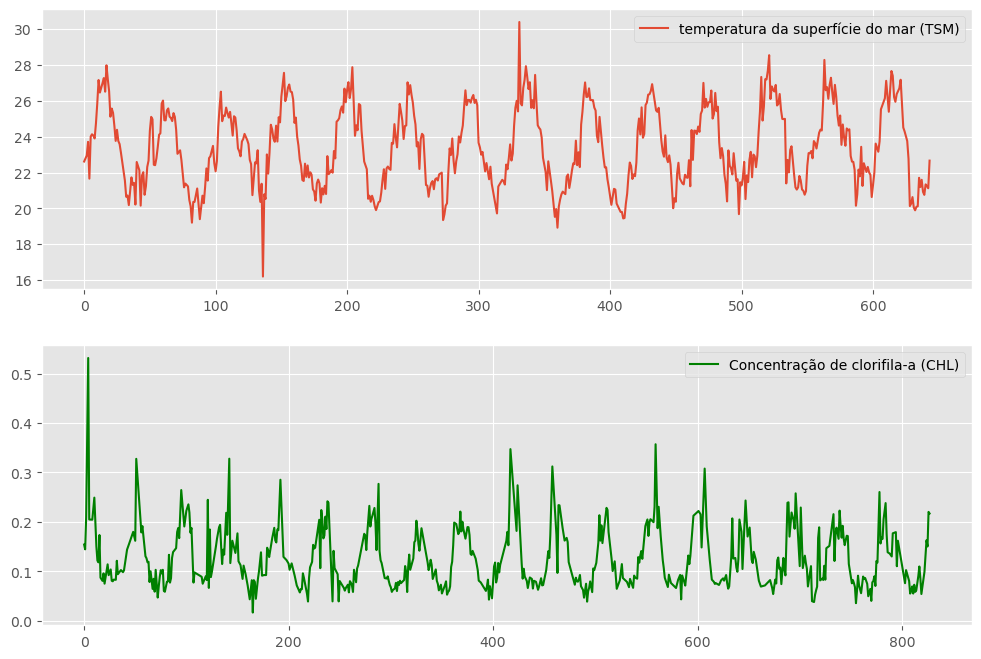
\includegraphics[width=1\linewidth]{lista4-2b]}
	\caption{Séries temporais de TSM e CHL}
	\label{fig:lista4-2b}
\end{figure}
	Analisando visualmente as séries, se nota que existe uma tendência ondulatória na mesma, comparando a tendência das duas, se nota que existe uma diferença de fase entre as duas séries, onde uma depressão de uma representa um pico na outra, a figura \ref{fig:lista4-2c} compara as séries utilizando o mesmo lag no eixo x para as duas, onde esse comportamento fica mais visível.
	
\begin{figure}[H]
	\centering
	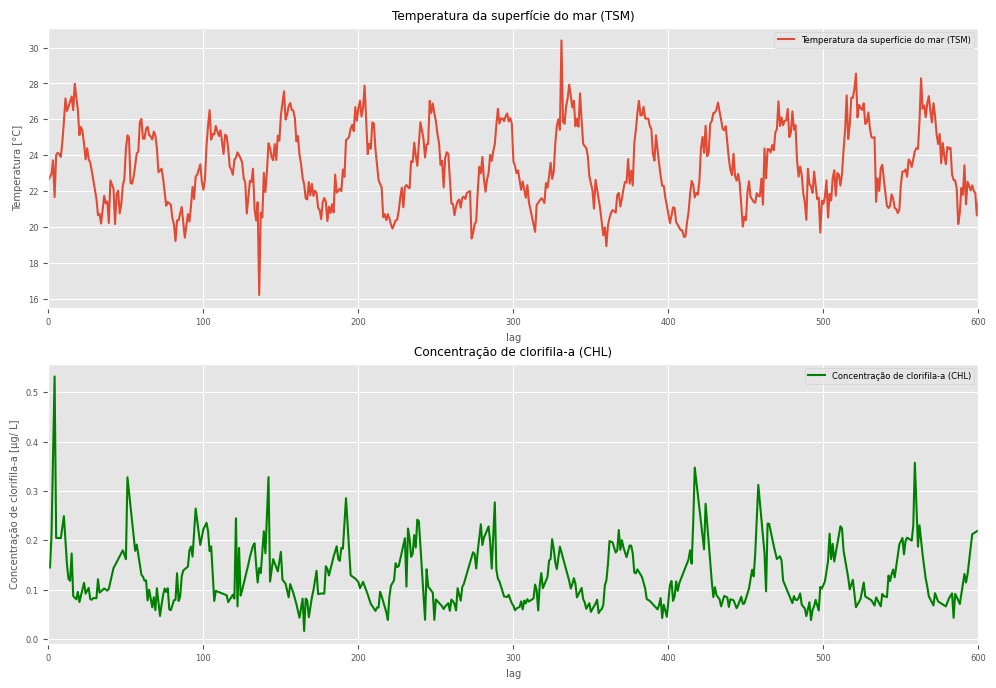
\includegraphics[width=1\linewidth]{lista4-2c}
	\caption{Séries temporais de TSM e CHL com o mesmo tamanho no eixo x}
	\label{fig:lista4-2c}
\end{figure}

Aplicando a função $\log_{10}$ na série de CHL, se obtém a figura \ref{fig:lista4-2d}
\begin{figure}[H]
	\centering
	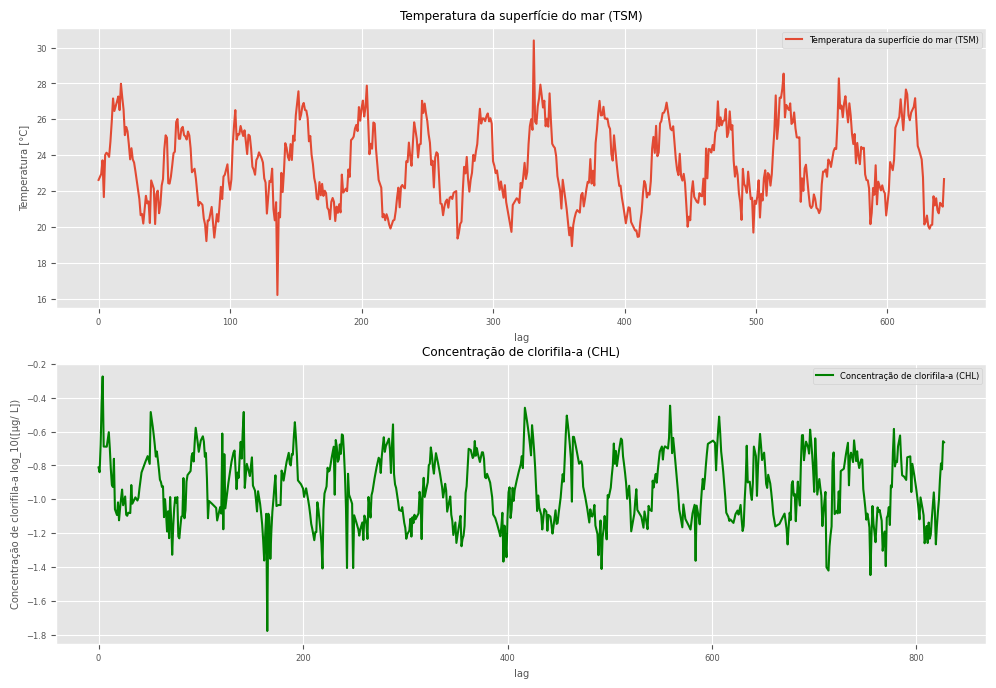
\includegraphics[width=1\linewidth]{lista4-2d}
	\caption{Séries temporais de TSM e de $\log_{10}(CHL)$}
	\label{fig:lista4-2d}
\end{figure}

Removendo a tendência se obtém a figura

\begin{figure}[H]
	\centering
	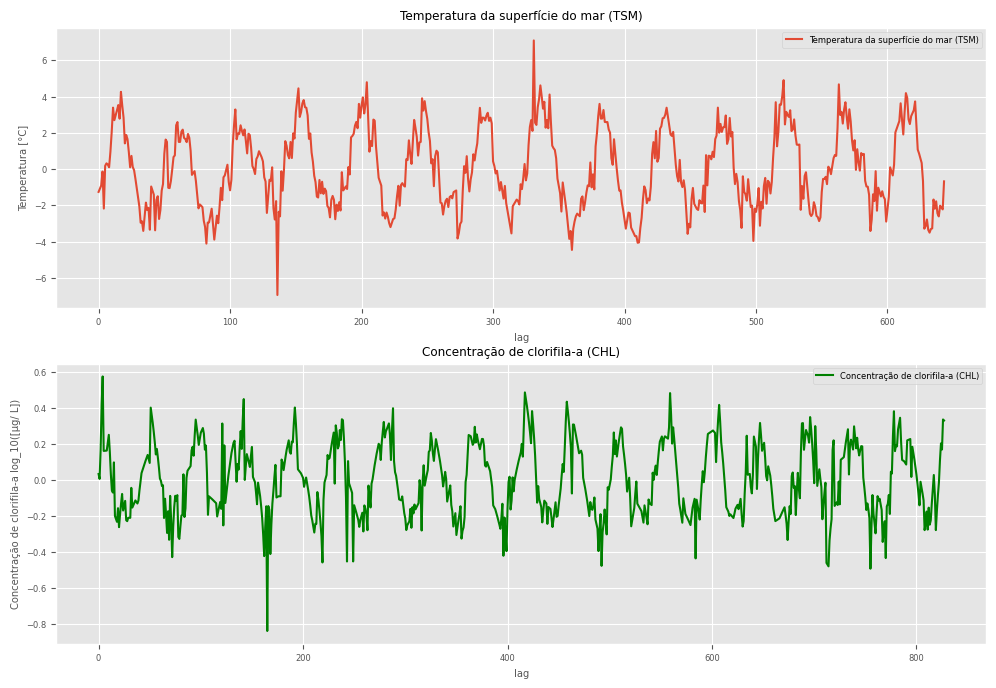
\includegraphics[width=1\linewidth]{lista4-2e}
	\caption{Anomalias nas séries temporais de TSM e de $\log_{10}(CHL)$}
	\label{fig:lista4-2e}
\end{figure}

A tabela \ref{Coeficientes para a clorifila-a } apresenta os coeficientes para as séries
\begin{table}[H]

\centering
\begin{tabular}{|c|c|c|c|c|}
	\hline
	Coeficientes & A & B & frequência & período \\
	\hline
	& 46.78 & 2.22 &  &  \\
	\hline
	&  0.23 & 0.21 &  6.2e$^{-3}$ & 161 \\
	\hline
	& 0.20 & 0.20 & 0.15 & 64.4   \\
	\hline
	& 0.16 & 0.16 & 0.10 & 9.6 \\
	\hline
	& 0.15 & 0.16 & 9.3e$^{-3}$ & 107.3 \\
	\hline
	& 0.15 & 0.14 & 1.5e$^{-3}$ & 644 \\
	\hline
\end{tabular}
\caption{Coeficientes para a clorifila-a}
\label{Coeficientes para a clorifila-a }
\end{table}

A tabela \ref{Coeficientes para a t} apresenta os coeficientes para as séries
\begin{table}[H]
\centering

\begin{tabular}{|c|c|c|c|c|}
	\hline
	Coeficientes & A & B & frequência & período \\
	\hline
	& 0.25 & 0.034 & 0.021 &  46\\
	\hline
	&   0.06 &0.014 &  0.043 & 23 \\
	\hline
	& 5.9e$^{-3}$& 5.8e$^{-3}$ & 0.036 & 27.6  \\
	\hline
	& 5.6e$^{-3}$ & 5.8e$^{-3}$ &  0.05 & 18\\
	\hline
	& 5.6e$^{-3}$& 5.3e$^{-3}$& 0.002 & 414 \\
	\hline
	& 5.1e$^{-3}$ & 5e$^{-3}$& 0.059 & 16.9 \\
	\hline
\end{tabular}
\caption{Coeficientes para a temperatura}
\label{Coeficientes para a t}
\end{table}
A figura \ref{fig:lista4-3d} mostra a reconstrução da Série para o $\log_{10}$ da clorofila.
\begin{figure}[H]
	\centering
	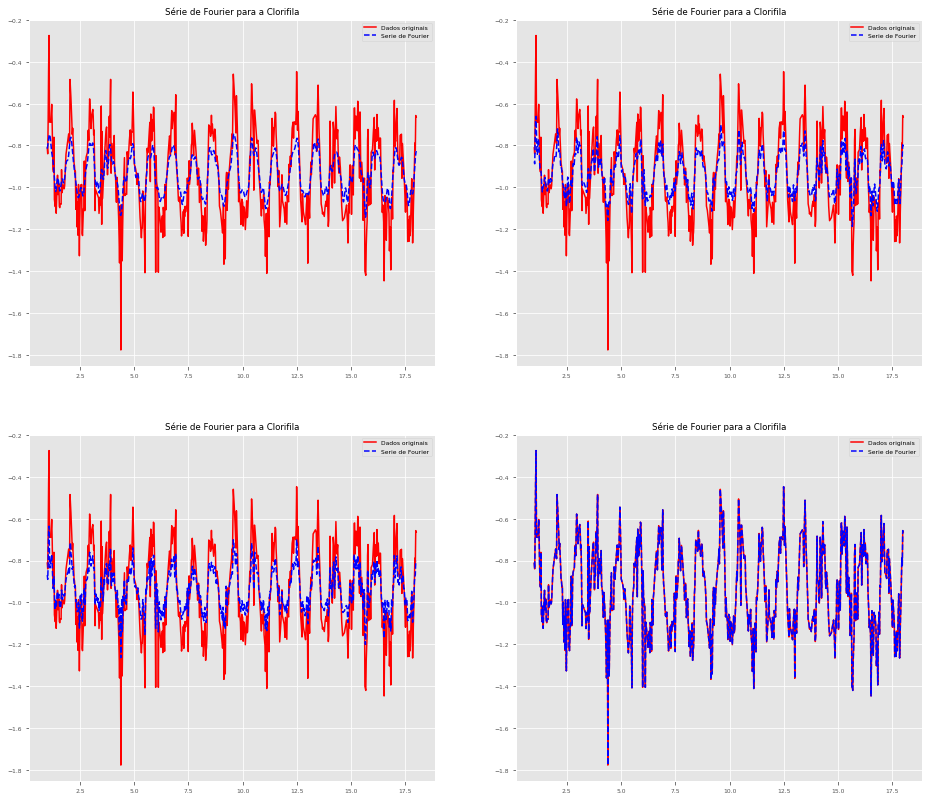
\includegraphics[width=1\linewidth]{lista4-3d}
	\caption{Reconstrução da Série para o $\log_{10}$ da Clorofila com o número de coeficientes variando.}
	\label{fig:lista4-3d}
\end{figure}
	
A figura \ref{fig:lista4-3e} mostra a reconstrução da Série para a temperatura.
\begin{figure}[H]
	\centering
	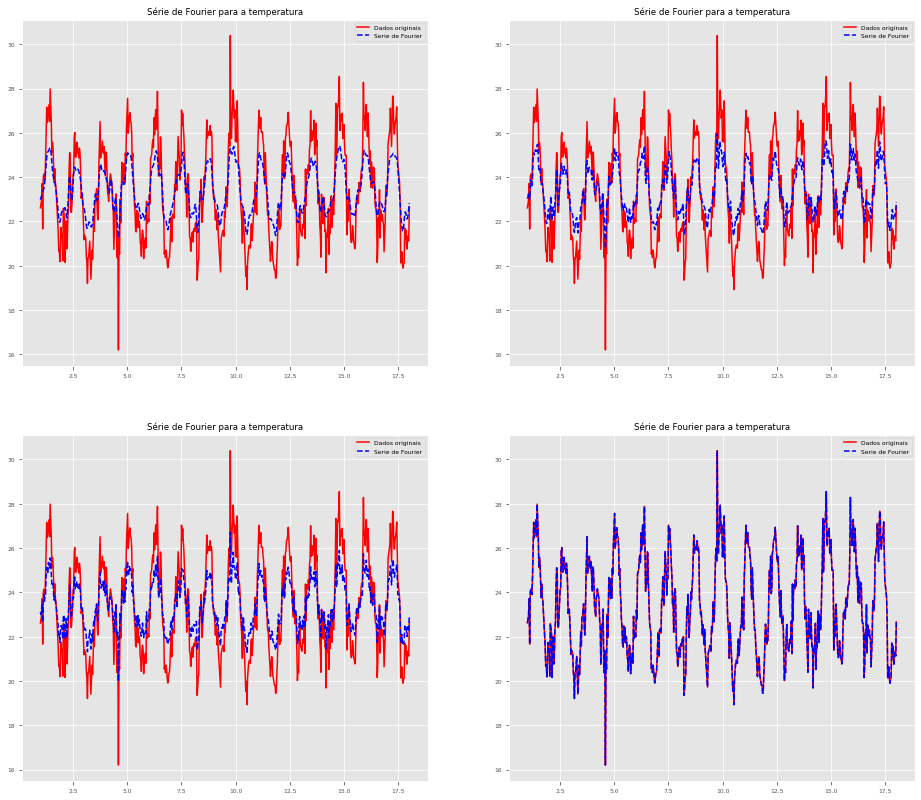
\includegraphics[width=1\linewidth]{lista4-3e}
	\caption{Reconstrução da Série para a temperatura com o número de coeficientes variando.}
	\label{fig:lista4-3e}
\end{figure}
\end{document}